\section[Системное описание предметной области и постановка задачи]{%
  СИСТЕМНОЕ ОПИСАНИЕ ПРЕДМЕТНОЙ \\
  ОБЛАСТИ И ПОСТАНОВКА ЗАДАЧИ
}\label{sec:system_spec}

\subsection{Выбор целевой мобильной платформы}

Для того, чтобы правильно выбрать целевую мобильную платформу
для разработки приложения, следует предварительно оценить состояние
и перспективы развития как рынка мобильных устройств связи в целом,
так и конкурирующих мобильных платформ в частности.
Под состоянием мобильной платформы имеется в виду
доля рынка, занимаемого данной платформой,
а под ее перспективами развития --- намерения компании-разработчика и
сообщества сторонних разработчиков эту платформу поддерживать.

В целом, современный рынок мобильных устройств можно охарактеризовать
как <<крупный>> и <<быстро развивающийся>>.
По данным ITU~\cite{itu_stat_phone}, представленным на
рисунке~\ref{fig:system_spec_stat_phones},
общее число мобильных устройств в мире возросло
более чем в три раза за последние десять лет
и составило более семи миллиардов.

\begin{figure}[h!]
  \centering
  \fcolorbox{gray}{white}{
    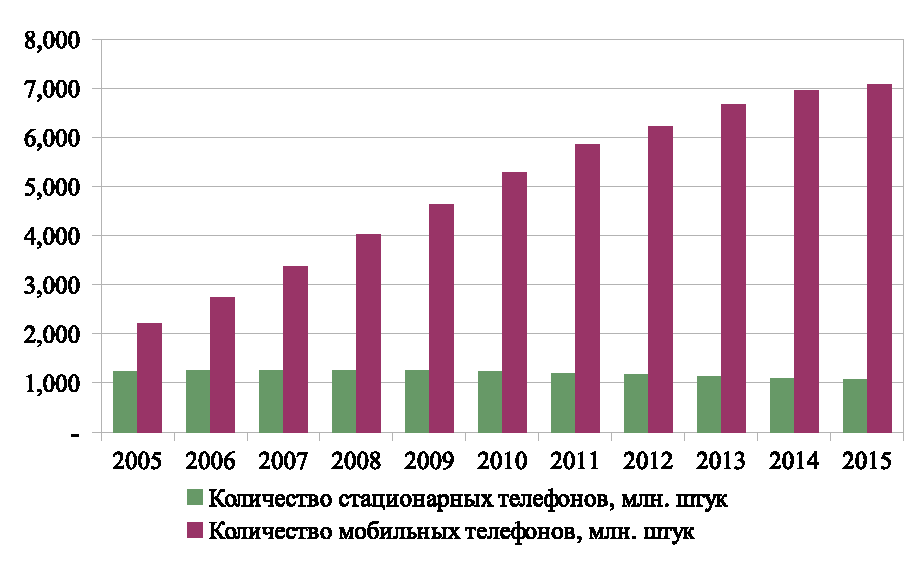
\includegraphics[width=140mm]{fig/system_spec_stat_phones.eps}
  }
  \caption{Динамика использования устройств связи}
  \label{fig:system_spec_stat_phones}
\end{figure}

По состоянию на 2015 год, на каждые 100 человек населения земного шара
приходится около 97 устройств мобильной связи.
Кроме того, можно с уверенностью утрерждать, что мобильная связь понемногу
вытесняет более традиционную проводную.

По данным компании Ericsson~\cite{ericsson_mobility_report},
в 2015 году было зарегистрировано использование около 3{,}4
миллиарда смартфонов для доступа в Интернет,
что составляет около 47\% от общего числа мобильных устройств.

Популярность различных мобильных платформ сравнивают, как правило,
по объемам продаж устройств, на которых они предустановлены.
В таблице~\ref{tbl:system_spec_stat_platforms} представлены данные
агенства Gartner~\cite{gartner_smartphone_stat} о динамике количества
проданных смартфонов, сгрупированных по различным мобильным платформам.

\begin{table}[h]
  \caption{
    Динамика количества проданных смартфонов под
    управлением различных операционных систем
  }\label{tbl:system_spec_stat_platforms}
    \begin{tabular}{| m{6cm} | c | c | c | c |}
      \hline
      \multirow{2}{*}{
      \parbox{6cm}{
      \smallskip
      \centering Операционная система
      \smallskip
      }
      }
      & \multicolumn{2}{c|}{
          \parbox{4.5cm}{
            \smallskip
            \centering Четвертый квартал 2014 года
            \smallskip
          }
        }
      & \multicolumn{2}{c|}{
          \parbox{4.5cm}{
            \smallskip
            \centering Четвертый квартал 2015 года
            \smallskip
          }
        } \\
      \cline{2-5}

      & млн. штук & \% & млн. штук & \% \\
      \hline

      Android &  279 & 76 & 325{,}4 & 80{,}7 \\
      \hline

      iOS &  75 & 20{,}4 & 71{,}5 & 17{,}7 \\
      \hline

      Windows & 10{,}5 & 2{,}8 & 4{,}5 & 1{,}1 \\
      \hline

      Blackberry & 1{,}7 & 0{,}4 & 0{,}9 & 0{,}3 \\
      \hline

      Другие & 1{,}3 & 0{,}4 & 0{,}9 & 0{,}2 \\
      \hline

      Всего & 367{,}5 & 100{,}0 & 400{,}6 & 100{,}0 \\
      \hline
    \end{tabular}
\end{table}
\vspace{-2.5mm}

Нетрудно заметить, что на данный момент наиболее популярной мобильной платформой
является Android --- мобильная платформа от компании Google,
занимающая на около 70\% рынка.
Кроме этого, из приведенных данных видно, что Android является единственной
платформой, относительная доля продаж мобильных устройств под управлением которой
за наблюдаемый период не сократилась.

Android позиционируется как бесплатная платформа для мобильных устройств любых
производителей, что позволяет снизить конечную стоимость, что, в свою очередь,
обуславливает высокую популярность платформы.
Android имеет открытый исходный код; авторы платформы
принимают патчи от сторонних разработчиков,
поэтому вокруг неё сформировалось достаточно активное сообщество.
Приведенные факты позволяют сделать вывод, что платформа Android является наиболее
перспективной для разработки мобильных приложений.

Весьма актуальным является вопрос выбора минимальной версии Android,
которая должна поддерживаться разрабатываемым мобильным приложением.
Дело в том, что различные версии этой платформы могут не обладать
полной обратной совместимостью. В связи с этим разработчикам приходится
соблюдать некоторый баланс между шириной охвата целевой аудитории приложения
и сложностью его разработки.
Действительно, с одной стороны, поддержка лишь новых версий Android сужает объем
потенциальной целевой аудитории, а поддержка максимально возможного числа версий
значительно усложняет общий процесс разработки и тестирования.
На рисунке~\ref{fig:system_spec_stat_android} представлены официальные
данные об относительной популярности различных версий
Android~\cite{google_stat_android}.

\begin{figure}[h!]
  \centering
  \fcolorbox{gray}{white}{
    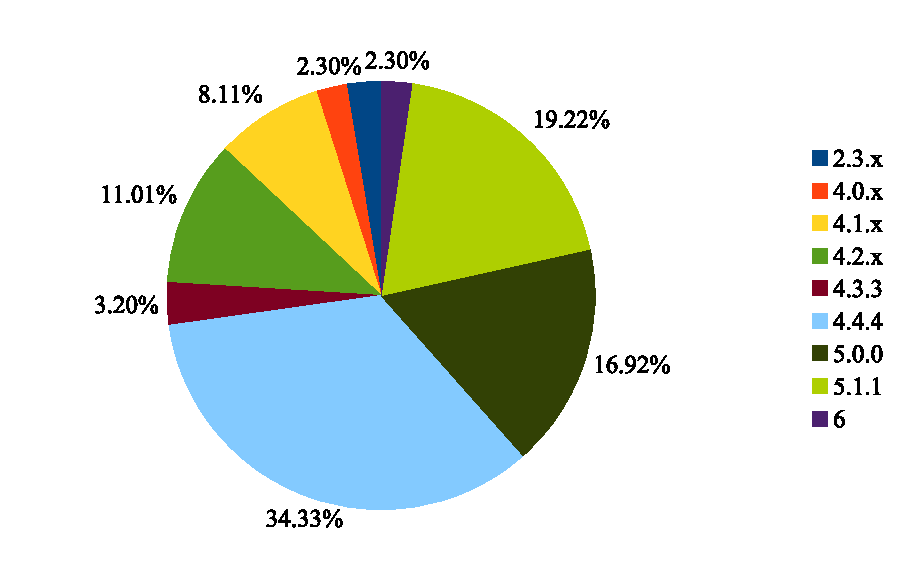
\includegraphics[width=140mm]{fig/system_spec_stat_android.eps}
  }
  \caption{Относительная популярность различных \\ версий платформы Android}
  \label{fig:system_spec_stat_android}
\end{figure}

Исходя из этих данных можно сделать вывод, что наиболее целесообразной
является разработка мобильного приложения для Android версии 4.0.x.
В этом случае оно будет доступно для 97\% пользователей Android,
а программный интерфейс платформы данной версии все еще остается
достаточно совместимым.


\subsection{Сравнительный анализ приложений-аналогов}
\label{subsec:system_spec_compare}

Для того, чтобы правильно выработать требования к разрабатываемому
программному обеспечению, следует предварительно сравнить
аналогичные решения, присутствующие на рынке.

Будем выбирать приложения для сравния следующим образом:
введем поисковую фразу, типичную для данной категории приложений,
например, <<money manager>>, в каталог мобильных приложений,
и выберем несколько приложений, расположившихся на верхних позициях
поисковой выдачи.
Данный подход призван сымитировать поведение типичного пользователя
Google Play Market, желающего установить себе подобное приложение,
при этом не обладающего какими-либо дополнительными информацией
о предмете поиска. Данным образом были выбраны следующие приложения,
расположенные в порядке выдачи:
\begin{itemize}
\item Monefy (автор: MonefyApp);
\item Money Manager Expense \& Budget (Realbyte Inc.);
\item Money Lover --- Money Manager (ZooStudio);
\item Money Manager Ex for Android (Android Money Manager Ex Prj);
\item AndroMoney (AndroMoney);
\item Expense Manager (Bishinews);
\item Money Manager Master (SMH17);
\item Money Manager (Praveen Thogarla).
\end{itemize}

Отметим, что как минимум пять приложений из этого списка поддерживаются
компаниями-разработчиками, что косвенно свидетельствует о сложности данных проектов.
Последний пункт списка на самом деле представляет собой два похожих друг
на друга одноименных приложения, разработанных индийскими программистами.

Определим основные категории сравнения мобильных приложений:
\begin{itemize}
\item базовые характеристики;
\item системные характеристики;
\item функциональные возможности;
\item пользовательского интерфейс.
\end{itemize}

Под базовыми характеристиками сравнения будем понимать
набор параметров приложения, доступных для оценки без установки приложения.
Как правило, они создают первое впечатление о приложении у конечного пользователя.
Системные характеристики представляют собой параметров функционирующего
приложения безотносительно выполняемых им функций.
Набор функциональных возможностей определяет способность приложения
удовлетворять запросы пользователя в контексте предметной области.
Пользовательский интерфейс влияет на удобство использования приложения в целом.

Рассмотрим категорию базовых характеристик приложения.
К числу таких характеристик относятся:
количество загрузок приложения, рейтинг приложения,
стоимость платной версии (если таковая имеется), ограничения бесплатной версии.
Результаты сравнения приложений по данным характеристикам приведены
в таблице~\ref{tbl:system_spec_cmp_basic}.

\begin{table} [h!]
  \caption{
    Базовые характеристики приложений-аналогов
  }\label{tbl:system_spec_cmp_basic}
    \begin{tabular}{| m{4cm} | c | c | c | c | c | c | c | c |}
      \hline
      \parbox{4cm}{
        \smallskip
        \centering Критерий \\ сравнения
        \smallskip
      }
      & \rotatebox[origin=c]{90}{
          \parbox{5cm}{
            Monefy
          }
        }
      & \rotatebox[origin=c]{90}{
          \parbox{5cm}{
            Money Manager \\ Expense \& Budget
          }
        }
      & \rotatebox[origin=c]{90}{
          \parbox{5cm}{
            Money Lover --- \\ Money Manager
          }
        }
      & \rotatebox[origin=c]{90}{
          \parbox{5cm}{
            Andro Money
          }
        }
      & \rotatebox[origin=c]{90}{
          \parbox{5cm}{
            Expense Manager
          }
        }
      & \rotatebox[origin=c]{90}{
          \parbox{5cm}{
            Money Manager Ex \\ for Android
          }
        }
      & \rotatebox[origin=c]{90}{
          \parbox{5cm}{
            Money Manager Master
          }
        }
      & \rotatebox[origin=c]{90}{
          \parbox{5cm}{
            Money Manager
          }
        } \\
      \hline

      Приблизительное \par количество \par загрузок \par приложения
      & \( 10^6 \)
      & \( 10^6 \)
      & \( 10^6 \)
      & \( 10^6 \)
      & \( 10^6 \)
      & \( 10^5 \)
      & \( 5 \cdot 10^3 \)
      & \( 10^3 \) \\
      \hline

      Рейтинг \par приложения
      & \( 4{,}5 \)
      & \( 4{,}5 \)
      & \( 4{,}5 \)
      & \( 4{,}7 \)
      & \( 4{,}3 \)
      & \( 4{,}4 \)
      & \( 4{,}6 \)
      & \( 4{,}5 \) \\
      \hline

      Ограничения \par бесплатной \par версии
      & Р\tablefootnote{принудительный показ рекламы.},
        Ф\tablefootnote{ограничения функциональности.}
      & Р, Ф
      & Р, Ф
      & Р
      & Р
      & \( - \)
      & Р, Ф
      & \( - \) \\
      \hline

      Стоимость \par
      платной версии, \$
      & \( 1{,}8 \)
      & \( 3{,}3 \)
      & \( 2{,}2 - 5 \)
      & \( 5 \)
      & \( 5 \)
      & \( - \)
      & \( 2{,}3 - 5 \)
      & \( - \) \\
      \hline
    \end{tabular}
\end{table}
\vspace{-2.5mm}

По приведенным данным можно сделать следующие выводы:
\begin{itemize}
  \item данный класс приложений пользуются высоким спросом;
  \item наиболее популярные приложения разрабатываются
    компаниями, а не частными лицами;
  \item монетизация приложений осуществляется в основном за
    счет принудительного показа рекламы в бесплатной версии приложения.
\end{itemize}

К системным характеристикам будем относить
размер установленного приложения и набор прав доступа,
требуемых для его функционирования.
Результат сравнения приведен в таблице~\ref{tbl:system_spec_cmp_system}.

\begin{table} [h!]
  \caption{
    Системные характеристики приложений-аналогов
  }\label{tbl:system_spec_cmp_system}
  \small{
    \begin{tabular}{| m{6.6cm} | c | c | c | c | c | c | c | c |}
      \hline
      \parbox{6.6cm}{
        \smallskip
        \centering Критерий \\ сравнения
        \smallskip
      }
      & \rotatebox[origin=c]{90}{
          \parbox{4.5cm}{
            Monefy
          }
        }
      & \rotatebox[origin=c]{90}{
          \parbox{4.5cm}{
            Money Manager \\ Expense \& Budget
          }
        }
      & \rotatebox[origin=c]{90}{
          \parbox{4.5cm}{
            Money Lover --- \\ Money Manager
          }
        }
      & \rotatebox[origin=c]{90}{
          \parbox{4.5cm}{
            Andro Money
          }
        }
      & \rotatebox[origin=c]{90}{
          \parbox{4.5cm}{
            Expense Manager
          }
        }
      & \rotatebox[origin=c]{90}{
          \parbox{4.5cm}{
            Money Manager Ex \\ for Android
          }
        }
      & \rotatebox[origin=c]{90}{
          \parbox{4.5cm}{
            Money Manager Master
          }
        }
      & \rotatebox[origin=c]{90}{
          \parbox{4.5cm}{
            Money Manager
          }
        } \\
      \hline

      Размер установленного \par приложения, Мб
      & \( 15{,}2 \)
      & \( 12{,}1 \)
      & \( 23{,}4 \)
      & \( 19{,}5 \)
      & \( 7{,}3 \)
      & \( 15{,}8 \)
      & \( 15{,}1 \)
      & \( 1{,}7 \) \\
      \hline

      Запрашиваемые права:
      & & & & & & & & \\

      -- доступ к карте памяти
      & +
      & +
      & +
      & +
      & +
      & +
      & +
      & \\

      -- доступ к Интернет
      & +
      & +
      & +
      & +
      & +
      & +
      & +
      & \\

      -- доступ к Google-аккаунту \par пользователя
      &
      &
      & +
      & +
      & +
      &
      & +
      & \\

      -- возможность управления \par вибратором
      &
      & +
      & +
      & +
      &
      & +
      &
      & \\

      -- возможность автоматического \par запуска приложения при \par старте системы
      &
      & +
      & +
      & +
      &
      & +
      &
      & \\

      -- возможность предотвращения \par
      автоматического перехода \par
      устройства в энергосберегающий \par
      режим
      &
      & +
      & +
      & +
      &
      &
      &
      & \\

      -- доступ к SMS пользователя
      &
      & +
      &
      & +
      & +
      &
      &
      & \\

      -- доступ к данным GPS
      &
      &
      & +
      &
      &
      &
      & +
      & \\

      -- доступ к телефонному модулю
      &
      & +
      &
      &
      &
      &
      & +
      & \\

      -- доступ к списку активных \par приложений
      &
      & +
      &
      &
      &
      &
      &
      & \\

      -- управление иконками \par рабочего стола
      &
      &
      & +
      &
      &
      &
      &
      & \\

      -- доступ к персональной \par информации
      &
      &
      &
      &
      &
      &
      & +
      & \\

      -- доступ к фотокамере
      &
      &
      &
      & +
      &
      &
      &
      & \\
      \hline
    \end{tabular}
  }
\end{table}
\vspace{-2.5mm}

По данным сравнения можно сделать следующие выводы:
\begin{itemize}
\item для работы большинства приложений необходимы доступ
  к карте памяти и сети Интернет;
\item приложения Monefy и Money Manager выгодно отличаются от конкурентов
  минимальным набором требуемых прав доступа;
\item некоторые приложения требуют использования прав,
  нетипичных для своего класса.
\end{itemize}

Установленное приложение должно занимать как можно меньше места и
требовать для работы как можно меньше прав доступа.
Поскольку стоимость ПЗУ достаточно низка, его объем для современных смартфонов
не является критическим ресурсом, поэтому размер установленного приложения не играет
существенной роли.
Иным образом обстоит дело с правами доступа:
с одной стороны, они могут быть необходимы для обеспечения работоспособности
базовых функций приложения (например, приложение, предоставляющее прогноз погоды,
должно иметь доступ в Интернет), использоваться для предоставления дополнительных
возможностей (приложение, предназначенное для обмена сообщениями,
может требовать доступ к карте памяти, где хранятся фотографии, для того, чтобы
прикреплять их к основному тексту).
С другой стороны, существует риск, что приложение, написанное недобросовестным
разработчиком, может использовать предоставленные предоставленные ему права
во вред владельцу устройства, (например, рассылать спам или передавать
персональные данные третьим лицам).
Поэтому набор запрашиваемых прав у мобильных приложений должен быть
минимально возможным.

В свете приведенных соображений требования приложений
Money Manager Expense \& Budget, Money Lover --- Money Manager,
Andro Money, Expense Manager и Money Manager Master доступа
к пользовательским SMS, данным навигации,
телефонному модулю выглядят весьма неоднозначено.
Особенно подозрительным представляется требование приложения
Money Manager Master доступа к персональным данным пользователя.

Для сравнения функциональных возможностей конкурирующих приложений
будем использовать набор типичных возможностей,
присущих приложениям данного класса.
Этот набор был составлен на базе личного пользовательского опыта.
Поясним некоторые из выбранных возможностей.
Возможность создания повторяющихся транзакций бывает удобна для
периодических статей прибыли и расхода денежных средств, например,
заработная плата, затраты на транспорт, оплата коммунальных услуг, и~т.~д.
Представление данных в виде диаграмм используется
для отображения изменения значений прибыли и затрат во времени,
а также для отображения относительной доли транзакций
каждой категории в общей сумме.
Функция ограничения величины расходов предупреждает пользователя
о превышении установленного лимита расходов определенной категории.
Результаты сравнения представлены в таблице~\ref{tbl:system_spec_cmp_func}.

\begin{table} [h]
  \caption{
    Функциональные возможности приложений-аналогов
  }\label{tbl:system_spec_cmp_func}
  \small{
  \begin{tabular}{| m{8cm} | c | c | c | c | c | c | c | c |}
      \hline
      \parbox{8cm}{
        \smallskip
        \centering Критерий \\ сравнения
        \smallskip
      }
      & \rotatebox[origin=c]{90}{
          \parbox{4.5cm}{
            Monefy
          }
        }
      & \rotatebox[origin=c]{90}{
          \parbox{4.5cm}{
            Money Manager \\ Expense \& Budget
          }
        }
      & \rotatebox[origin=c]{90}{
          \parbox{4.5cm}{
            Money Lover --- \\ Money Manager
          }
        }
      & \rotatebox[origin=c]{90}{
          \parbox{4.5cm}{
            Andro Money
          }
        }
      & \rotatebox[origin=c]{90}{
          \parbox{4.5cm}{
            Expense Manager
          }
        }
      & \rotatebox[origin=c]{90}{
          \parbox{4.5cm}{
            Money Manager Ex \\ for Android
          }
        }
      & \rotatebox[origin=c]{90}{
          \parbox{4.5cm}{
            Money Manager Master
          }
        }
      & \rotatebox[origin=c]{90}{
          \parbox{4.5cm}{
            Money Manager
          }
        } \\
      \hline

      Управление данными:
      & & & & & & & & \\

      -- ведение нескольких счетов
      & +
      & +
      & +
      & +
      & +
      & +
      & +
      & \\

      -- редактирование категорий учета
      & *\tablefootnote{в платной версии.}
      & +
      & +
      & +
      & +
      & +
      & +
      & + \\

      -- создание повторяющихся транзакций
      &
      & +
      & +
      & +
      & +
      & +
      & +
      & \\

      -- поддержка нескольких валют
      &
      & +
      & +
      & +
      & +
      & +
      & +
      & \\
      \hline

      Представление данных:
      & & & & & & & & \\

      -- группировка данных по времени
      & +
      & +
      & +
      & +
      & +
      & +
      & +
      & + \\

      -- группировка данных по категориям
      & +
      & +
      & +
      & +
      & +
      & +
      & +
      & + \\

      -- группировка данных по типу транзакций
      &
      & +
      & +
      &
      & +
      & +
      & +
      & + \\

      -- представление данных в виде диаграмм
      & +
      & +
      & +
      & +
      & +
      & +
      & *
      & + \\

      \hline

      Дополнительные возможности:
      & & & & & & & & \\

      -- резервное копирование
      & +
      & +
      & +
      & +
      & +
      & +
      &
      & \\

      -- ограничение величины расходов
      & +
      & +
      & +
      & +
      & +
      & +
      &
      & \\
      \hline

      -- настройка напоминаний \par
      о необходимости ввода данных
      &
      &
      & +
      & +
      &
      &
      &
      & \\

      -- поиск транзакций
      &
      & +
      & +
      & +
      &
      & +
      &
      & \\

      -- парольная защита доступа к данным
      & +
      & +
      &
      & +
      & +
      & +
      &
      & \\

      -- экспорт/импорт данных из файла
      & +
      & *
      & +
      & +
      & +
      & +
      &
      & \\

      -- синхронизация данных с сервером
      & +
      & *
      & +
      & +
      & +
      & +
      &
      & \\
      \hline
    \end{tabular}
  }
\end{table}

Рассматриваемые приложения можно разделить на три группы в
зависимости от соотношения количества поддерживаемых
возможностей и удобства пользовательского интерфейса.
Первая группа приложений (куда входят Money Manager Expense \& Budget,
Money Lover --- Money Manager, Andro Money, Expense Manager,
Money Manager Ex for Android)
имеют широкий набор функций и большое количество настроек.
Вторая группа приложений, состоящая из Monefy и Money Manager Master,
имеют меньший набор возможностей, но зачастую более удобный интерфейс.
Третья группа представлена предельно простым в использовании приложением Money Manager,
имеющим минимальный набор функций.

Поскольку сравнение пользовательских интерфейсов программных продуктов
является делом заведомо субъективным, ограничимся следующими критериями:
соответствие дизайна рекомендациям Google, наличие возможности управления жестами,
наличие локализаций приложения.

Наличие различных локализаций приложения значительно расширяет потенциальную
аудиторию пользователей приложения, позволяя пользоваться им на родном языке.
В таблице~\ref{tbl:system_spec_cmp_interface} представлен результат сравнения
пользовательских интерфейсов рассматриваемых приложений.

\begin{table} [h!]
  \caption{
    Пользовательский интерфейс приложений-аналогов
  }\label{tbl:system_spec_cmp_interface}
    \begin{tabular}{| m{6.9cm} | c | c | c | c | c | c | c | c |}
      \hline
      \parbox{6.9cm}{
        \smallskip
        \centering Критерий \\ сравнения
        \smallskip
      }
      & \rotatebox[origin=c]{90}{
          \parbox{4.5cm}{
            Monefy
          }
        }
      & \rotatebox[origin=c]{90}{
          \parbox{4.5cm}{
            Money Manager \\ Expense \& Budget
          }
        }
      & \rotatebox[origin=c]{90}{
          \parbox{4.5cm}{
            Money Lover --- \\ Money Manager
          }
        }
      & \rotatebox[origin=c]{90}{
          \parbox{4.5cm}{
            Andro Money
          }
        }
      & \rotatebox[origin=c]{90}{
          \parbox{4.5cm}{
            Expense Manager
          }
        }
      & \rotatebox[origin=c]{90}{
          \parbox{4.5cm}{
            Money Manager Ex \\ for Android
          }
        }
      & \rotatebox[origin=c]{90}{
          \parbox{4.5cm}{
            Money Manager \\ Master
          }
        }
      & \rotatebox[origin=c]{90}{
          \parbox{4.5cm}{
            Money Manager
          }
        } \\
      \hline

      Соответствие дизайна \par рекомендациям Google
      &
      & +
      & +
      &
      &
      & +
      &
      & + \\
      \hline

      Возможность управления \par жестами
      & +
      &
      & +
      & +
      & +
      & +
      &
      & \\
      \hline

      Наличие локализаций
      & +
      &
      & +
      &
      & +
      & +
      &
      & \\
      \hline
    \end{tabular}
\end{table}

Результаты сравнения свидетельствуют о том, что наиболее проработанным
пользовательским интерфейсом обладают приложения
Money Lover --- Money Manager и Money Manager Ex for Android.

Общие результаты анализа показывают, что рассмотренные приложения
можно разделить на три группы.
Приложения первой группы имеют большую аудиторию пользователей,
развитую функциональность и большое количество настроек.
Все эти приложения являются коммерческими,
бесплатные версии которых показывают рекламные баннеры.
Сюда относятся Monefy, Money Manager Expense \& Budget,
Money Lover --- Money Manager, Andro Money, Expense Manager.
Приложения второй группы также имеют развитую функциональность,
но меньшую аудиторию пользователей.
Во вторую группу входят такие приложения, как
Money Manager Ex for Android и Manager Master.
Третья группа представлена приложением Money Manager,
обладающим небольшой популярностью и имеющим весьма скромный набор функций.
Отметим, что данное приложение является бесплатным,
не содержит рекламы и имеет простой пользовательский интерфейс.

Мобильное приложение, разрабатываемое в рамках данного проекта,
следует причислить к третьей группе приложений,
поскольку в автором предполагается проектирование и реализация лишь
минимального числа наиболее частоиспользуемых функций.
Кроме этого, автор приложения не преследует цели получения
коммерческой выгоды от его реализации и использования конечными пользователями.

\subsection{Постановка задачи проектирования}
\label{subsec:system_spec_task}

Требуется выполнить проектирование и
программную реализацию мобильного приложения, выполняющего учет и представление
финансовой информации пользователя.
Данное приложение должно работать под управлением мобильной ОС Android 4.0.x,
распространяться на бесплатной основе и не иметь ограничений функциональности.
Кроме этого, оно должно иметь небольшой размер, не требовать доступа к сети Интернет
и к личным данным пользователя.

Приложение должно иметь следующий набор функций:
\begin{itemize}
  \item возможность веденияч нескольких счетов;
  \item возможность редактирование категорий учета;
  \item поддержка нескольких валют учета;
  \item возможность группировки данных по дате и категориям учета.
\end{itemize}
Ввод финансовых данных должен осуществляться как в ручном,
так и в полуавтоматическом режиме с использованием фотокамеры мобильного устройства.
Приложение должно предусматривать вывод данных в наглядной форме и иметь
русскую локализацию, а также удобный пользовательский интерфейс,
выполненный в соответствии с рекомендациями Google.
